\chapter{Implementation}\label{ch:implementation}

\section{Koncept}

\section{Architectur}

\section{Message protocol}
In unserer Implementation wird, sobald eine neuer Besucher der Webseite hinzukommt, sofort ein DataChannel, mittels WebRTC, STUN, ICE und Signaling server zu allen anderen aktiven Besuchern aufgebaut. Über diesen werden zu zwei Zeitpunkten Informationen darüber ausgetauscht, welche Ressourcen bei dem jeweiligen Nutzer vorliegen: Direkt nach Aufbau des DataChannels und immer dann, wenn ein Nutzer eine neue Ressource (aus dem Internet oder lokal) geladen und in seinem Cache gespeichert hat:

\begin{figure}[!h]
	\centering
	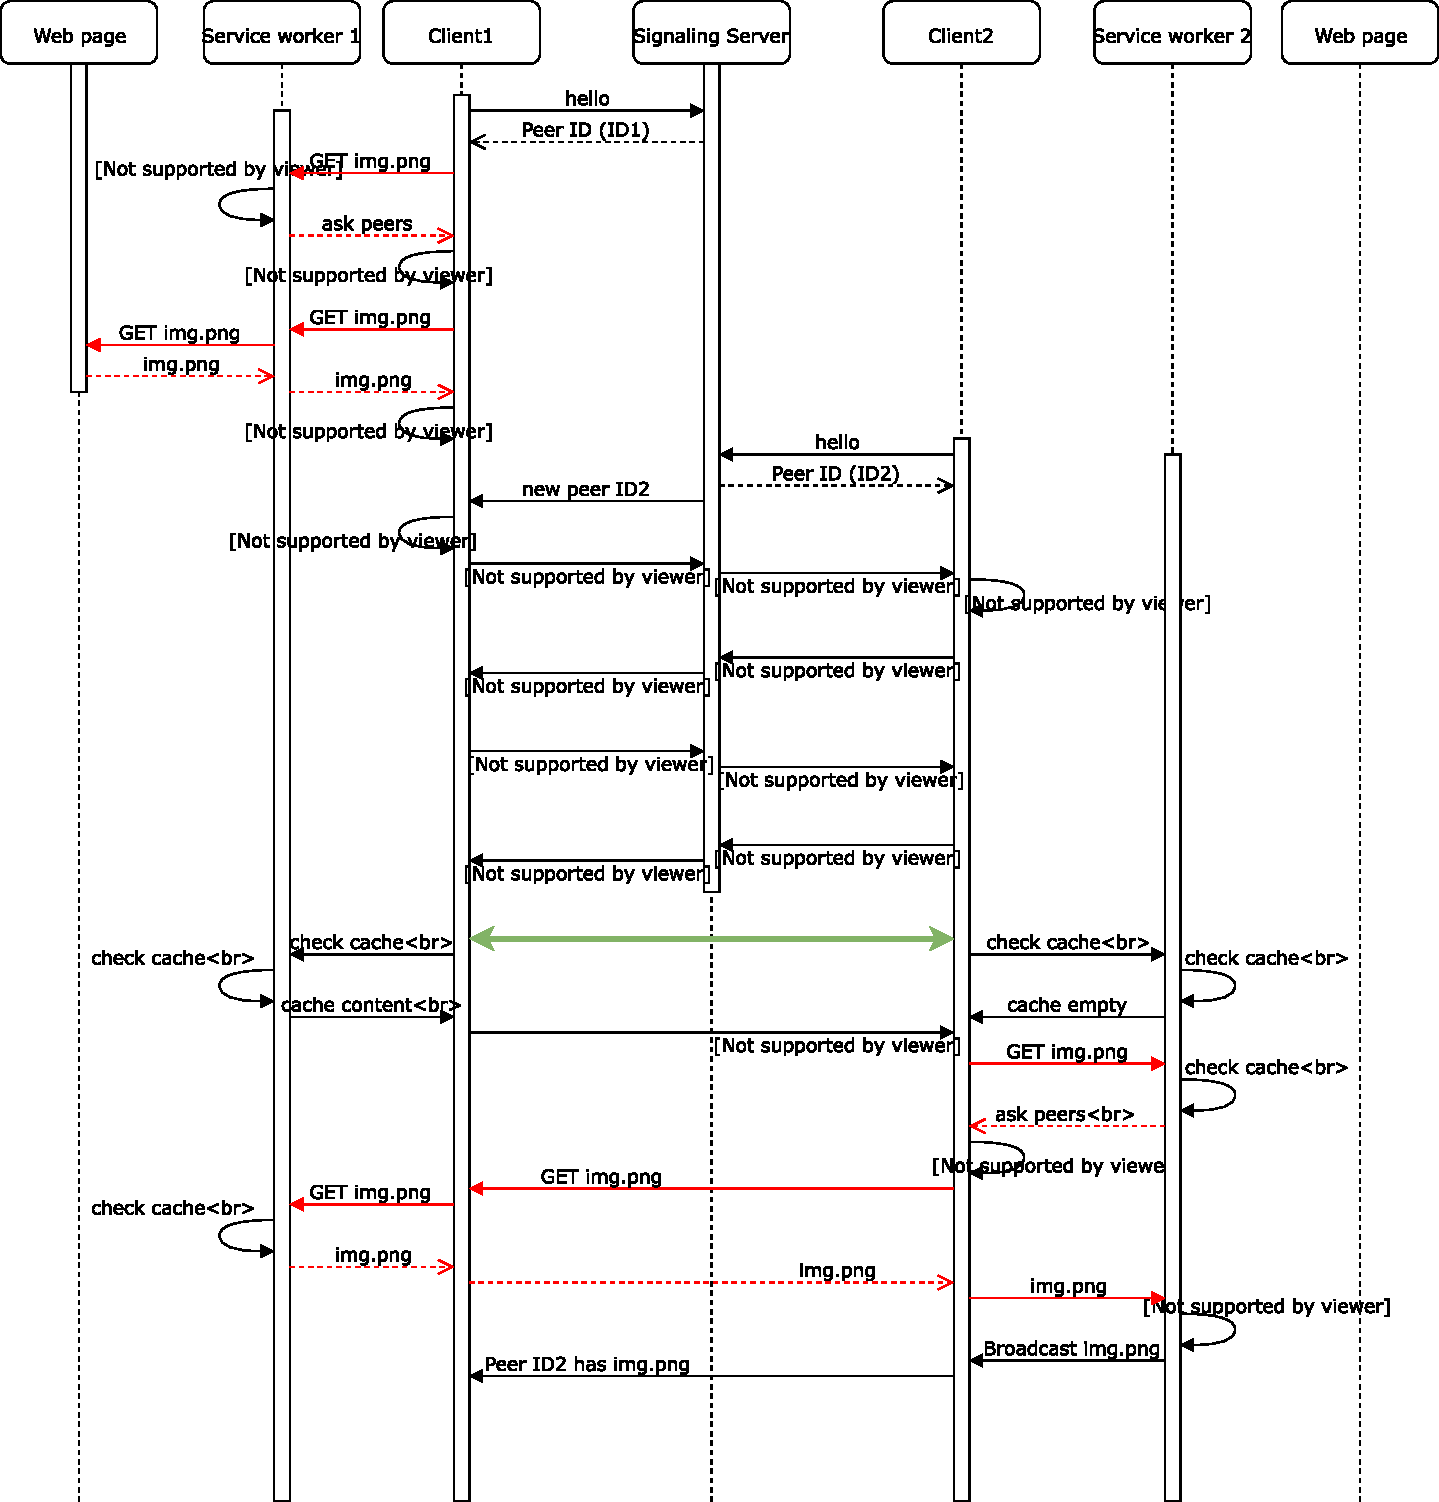
\includegraphics[width=0.8\textwidth]{figures/SequenceDiagram}
	\caption[A Figure Short-Title]{A Figure Title}
	\label{fig:sequenceDiagram}
\end{figure}

Client 1 (C1) ist der erste der die Webseite aufruft. Er registriert sich beim Signaling server und fragt im Anschluss img.png an (rot). Da noch niemand anders auf der Seite ist von dem er die Ressource bekommen könnte und er zudem die Ressource nicht in seinem Cache hat, wird img.png über das Internet vom Webserver geladen. Client 2 (C2) ruft nun ebenfalls die Webseite auf und registriert sich beim Signaling server. Dieser benachrichtigt C1, dass ein neuer Teilnehmer registriert wurde, woraufhin C1 einen Verbindungsaufbau zu C2 einleitet. Steht die direkte Verbindung zwischen C1 und C2 (grün), teilt C1 C2 den Inhalt seines aktuellen Caches mit. Fragt C2 img.png an (rot), weiß er so, dass er diese von C1 anfragen kann. Hat er img.png erhalten, teilt er allen anderen Teilnehmern (in diesem Fall nur C1) mit, dass auch er jetzt img.png als Ressource in seinem Cache hat

\section{Data serialization}

\section{Reusability}
